\documentclass[twocolumn,amsmath,amssymb,pra, floatfix]{revtex4-2}
\usepackage[utf8]{inputenc}
\usepackage{graphicx}
\graphicspath{ {Images/} }
\usepackage{siunitx}
\usepackage{hyperref}
\usepackage{caption}
%\usepackage{gensymb}
\usepackage{float}
\usepackage{comment}
\usepackage{bm}

\begin{document}

\title{The Chaotic Pendulum}
\author{Timothy O'Gallagher, Jun Sung}
\date{April 29 2021}

\begin{abstract}
The purpose of this lab is to study and analyze the differences between non-chaotic and chaotic motion. 
The main method used to study this difference was through a dual-pulley pendulum, and we measured the 
angular position with time as well as the angular velocity with respect to the angular position.
From this, we were able produce phase plots, Poincar\'{e} plots, and FFT plots. These plots allowed us to
analyze the difference between non-chaotic (both undriven and driven as well as damped) and chaotic behavior, and it allowed for us to also calculate
the Lyapunov exponent for each behavior. The results that we got were promising -- the non-chaotic motion resulted in a Lyapunov exponent of $-5.94 \times 10^{-3} \pm 4.38 \times 10^{-3}$, and the chaotic motion resulted in a Lyapunov constant of $1.35 \pm 4.38 \times 10^{-3}$. These results do indeed tell us that our measured non-chaotic motion was non-chaotic, and our measured chaotic motion was chaotic. We also looked into the potential wells of our pendulum and found two wells -- as expected with how our apparatus was set up.

\end{abstract}

\maketitle

\section{Introduction}
Periodic motion is one of the most fundamental types of motion in physics, with the best example being the harmonic oscillator. However, there are some experimental conditions where the motion ceases to be periodic and takes on a more unpredictable, sporadic nature. This type of seemingly unpredictable motion, which is also characterized by extreme sensitivity to initial conditions, is called chaos and it arises in a number of scientific contexts. The goal of this experiment is to investigate the properties of chaotic motion with a pendulum, and to examine how experimental parameters, such as the damping, the amplitude, the driving force, and the initial conditions, influence the motion as well as the transition between periodic and chaotic motion. 

Our apparatus for this experiment consists of an aluminum disk and a point mass on the edge, tied to two springs that both have a spring constant of $k$ -- Confer Figure \ref{fig:apparatus_schematic}. One of the springs is tied to a driving motor that rotates with angular velocity $\Omega$. We can define the drive phase as $\phi$, and we can say that $\phi = \Omega t$. If we say that $A$ is the distance from the rotation axis to the tip of the driving motor, then we can approximate the displacement of the driven spring as $d=A \cos\phi$. We use this to compute the external torque on the system.  

To derive the equations of motion, we need to find the torque on the system. The gravitational force on the point mass is $mg$, with $m$ as the value of the point mass. If $\theta$ is the angular position of the point mass with respect to the vertical, then we can say that the gravitational torque is $\vec{\tau} = \vec{r}\times\vec{F} = mgl \sin{\theta}$. Here, we define $l$ to be the radius of the aluminum disk (distinct from the radius of the pulley, which we denote by $r$). Additionally, there are torques from the springs. The force from a single spring on the pulley of radius $r$ is $-kr\theta$, where $r\theta$ is the displacement of the spring, as well as the arc length of the angular position of the mass. The force from both is $-2kr\theta$, and the torque is $-2kr^{2}\theta$. From the other end of the driven spring, there is an additional force in the downward direction on the pulley from the motor. The displacement is $d$ (as depicted in Figure \ref{fig:apparatus_schematic}), which gives a force of $kd$ and a torque of $krd$. To damp the system, we bring a magnet close to the aluminum disk.
The magnet will exert a torque on the disk, and we can model it as $-b\omega$, where $\omega$ is the angular velocity of the disk. The final torque on the system comes from the friction from the rotating axle. We can model such a torque similarly to what we did with the magnet and assume that the torque caused by friction is constant, say of magnitude $b'$. Since the torque caused by friction opposes the motion, we can model this torque by $-b' \mathrm{sgn}\omega$, where $ \mathrm{sgn}\omega = \frac{\omega}{\mid\omega\mid}$. 

\begin{figure}[H]
    \centering
    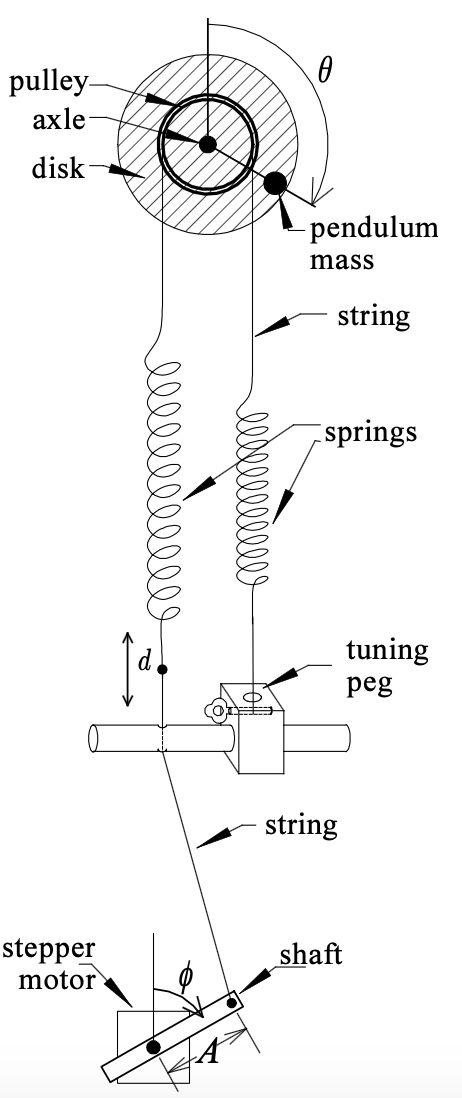
\includegraphics[width = 0.4\linewidth]{images/apparatus_schematic.png}
    \caption{A labelled schematic of our pendulum oscillator}
    \label{fig:apparatus_schematic}
\end{figure}

Now that we have derived the torque on the system, we can apply Newton's second law of rotation as follows:

\begin{equation}
    I\ddot{\theta}=-2kr^{2}\theta+krA\cos{\phi}+mgl\sin{\theta} - b\omega -b'  \mathrm{sgn}{\omega}
    \label{eq:1}
\end{equation}

Here, $I$ is the moment of inertia for the system. The disk and pulley system have moment of inertia $I_{0}$, the point mass has moment of inertia $I_{m}$, and the total moment of inertia is given by $I = I_{m} + I_{0} + ml^{2}$. Given this, we can make the following substitutions to simplify the equation of motion:

\begin{equation}
    \Gamma = \frac{b}{I}
    \label{eq:2}
\end{equation}

\begin{equation}
    \Gamma' = \frac{b'}{I}
    \label{eq:3}
\end{equation}

\begin{equation}
    \kappa = \frac{2kr^{2}}{I}
    \label{eq:4}
\end{equation}

\begin{equation}
    \mu = \frac{mgl}{I}
    \label{eq:5}
\end{equation}

\begin{equation}
    \epsilon = \frac{krA}{I}
    \label{eq:6}
\end{equation}

An additional simplification is that we write the equation of motion as three first order differential equations. The final set of equations is:

\begin{equation}
    \dot{\theta} = \omega
    \label{eq:7}
\end{equation}

\begin{equation}
    \dot{\omega} = -\Gamma\omega - \Gamma' \mathrm{sgn}\omega - \kappa\theta + \mu \sin{\theta} + \epsilon \cos{\phi}
    \label{eq:8}
\end{equation}

\begin{equation}
    \dot{\phi} = \Omega
    \label{eq:9}
\end{equation}

With these equations of motion, there are three ways we can graph the oscillations. One method is to simply plot $\theta$ vs. time. Another way is to plot $\omega$ vs. $\theta$. The third method is called a Poincar\'{e} section. The first two methods are self-explanatory in terms of what they represent. However, we will take this time to discuss the third method.

In order to understand how a Poincar\'{e} section is constructed, consider a three-dimensional phase space with coordinates $\omega$, $\theta$, and $\phi$. With this coordinate system, $phi$ is the azimuthal coordinate, with each $\phi$ value corresponding to a different $\theta$-$\omega$ plane. Each $\theta$-$\omega$ plane corresponding to a particular value of $\phi$ is called a Poincar\'{e} section.

We can think of the three equations of motion (equations \ref{eq:7}-\ref{eq:9}) as a vector function acting on a three dimensional point in phase space. Figure \ref{fig: phase space plot} illustrates the coordinate system in this space.

\begin{figure}[H]
    \centering
    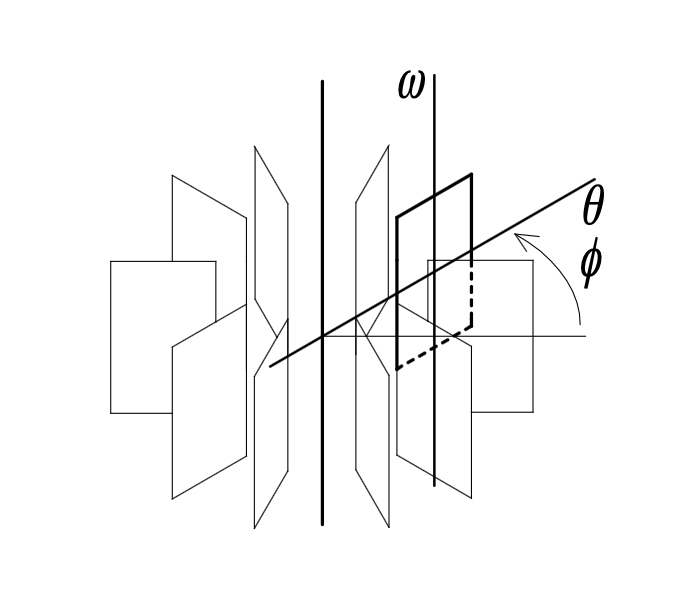
\includegraphics[ width = 0.5\linewidth ]{images/phase_space_plot.PNG}
    \caption{The Coordinate System that would be used to plot the system in three dimensions}
    \label{fig: phase space plot}
\end{figure}

To give an example of how a plot of our system may look, consider the oscillator with driven damped sinusoidal oscillations. Here, the $\theta$ vs. time graph would look like as shown in Figure \ref{fig: sine linear theta vs time plot}

\begin{figure}[H]
    \centering
    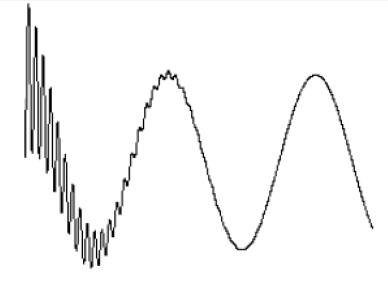
\includegraphics[ width = 0.5\linewidth ]{images/theta_vs_time_sine_wave.PNG}
    \caption{The theta vs. time plot of linear sinusoidal driven, damped oscillations}
    \label{fig: sine linear theta vs time plot}
\end{figure}

Whereas the graph in the three dimensional phase space would look like as shown in Figure \ref{fig: sine phase space plot}. 

\begin{figure}[H]
    \centering
    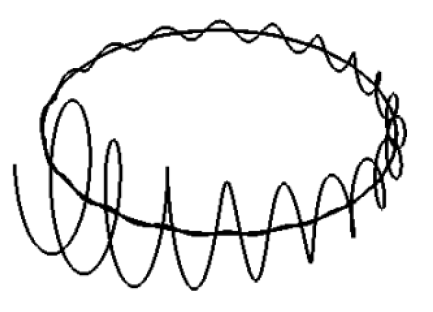
\includegraphics[width = 0.5\linewidth]{images/phase_space_sine_wave.PNG}
    \caption{The phase space plot of linear, sinusoidal, driven, damped oscillations}
    \label{fig: sine phase space plot}
\end{figure}

We refer to the plot of the system in three dimensional phase space as the trajectory. We can see that this trajectory reaches a steady state, where it repeats the same pattern through time. This steady state is shown in Figure \ref{fig: sine wave phase space attractor}

The set of points that define the steady state is called the attractor, since it is the set of points that the trajectory moves toward in time. 

In our second method of plotting the oscillations, which we specified as plotting $\omega$ vs. $\theta$, we would predict from this theory that the curve would take a spiral shape toward the origin. In this two-dimensional projection, the origin is the attractor. We expect the Poincare section of this trajectory to be a single point, because, once the initial transient motion dies out, the point in each $\omega$-$\theta$ plane is the same at each periodically recurring instance of a given $\phi$ coordinate, because of the steady state.

\begin{figure}
    \centering
    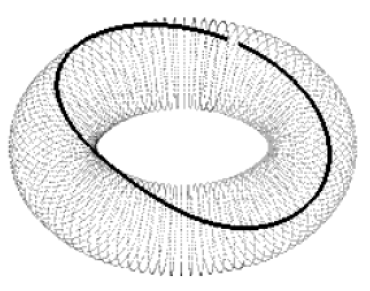
\includegraphics[width = 0.5\linewidth]{images/attractor_sine_wave.png}
    \caption{The steady state of the trajectory in phase space}
    \label{fig: sine wave phase space attractor}
\end{figure}

Chaotic motion is characterised by motion that never arrives at a steady state. The Poincare section and the $\omega$ vs $\theta$ come in handy when analyzing this type of motion because the $\theta$ vs time plots are often too complex and sporadic to glean any useful information. Theory and past experiment predict that the Poincare section for chaotic motion looks like as shown in Figure \ref{fig: Chaotic Poincare section graphs}:

\begin{figure}[H]
 \centering
 \begin{minipage}{0.7\linewidth}
    \centering 
    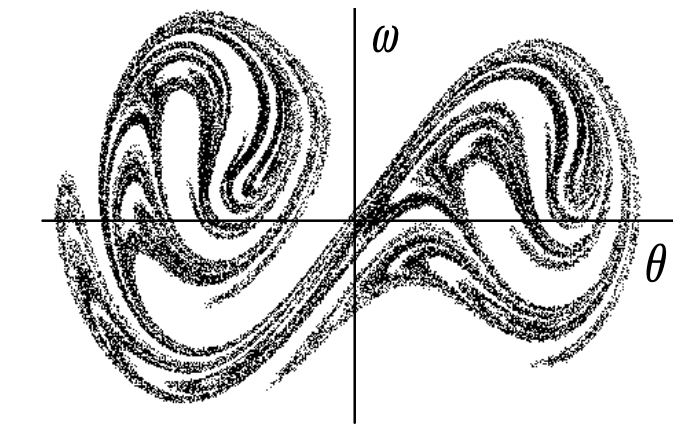
\includegraphics[width = 0.7\linewidth]{images/Poincare_section_chaos_.png}
    \caption*{(a) Poincare section for chaotic motion}
 \end{minipage}%
 \\[2mm]
  \begin{minipage}{0.7\linewidth}
    \centering 
    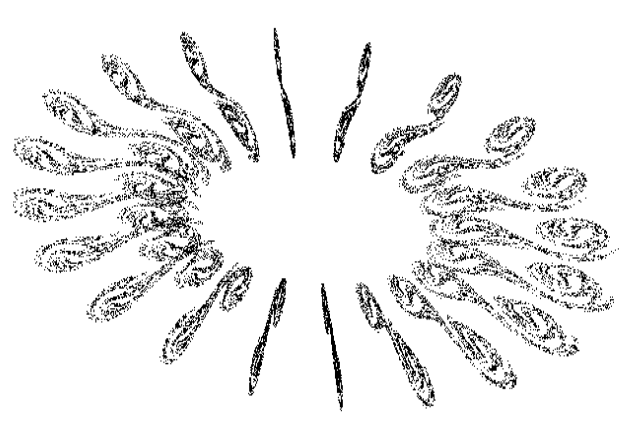
\includegraphics[width = 0.7\linewidth]{images/Poincare_section_chaos_3D.png}
    \caption*{(b) Series of chaotic Poincare sections in three dimensions}
 \end{minipage}%
 \caption{Visual representations of the chaotic Poincar\'{e} section}
 \label{fig: Chaotic Poincare section graphs}
\end{figure}

One interesting and important into to note is that if you zoom in on a small section of a Poincare section for chaotic motion, you would find that the pattern repeats on smaller scales as you zoom in, and this continues indefinitely. This is called fractal geometry, and attractors with fractal geometry are referred to as strange attractors. 

Our goal is to use our three methods of plotting the oscillations to examine the trends from steady state towards chaotic strange attractors as several system parameters are varied. Furthermore, we determine the Lyapunov exponents for both non-chaotic and chaotic motion to verify that what we have is indeed non-chaotic or chaotic motion. As for how we can calculate the Lyapunov exponents, we consider two phase points that are very close together, say $\mathbf{u}$ and $\mathbf{u}'$ and define their difference to be 
\begin{equation}
    \delta \mathbf{u} = \mathbf{u}' - \mathbf{u}
    \label{eq:10}
\end{equation}

Note that $\mathbf{u}$ and $\mathbf{u}'$ are our initial points, and our goal is to see how the distances between these two points vary as we let time to vary. With enough points, we can determine a model for this time dependence and have the following to be the best representation:

\begin{equation}
    \lvert \delta \mathbf{u}( t ) \rvert
    =
    \lvert \delta \mathbf{u}( 0 ) \rvert \exp(\lambda t)
    \label{eq:11}
\end{equation}

Where $\lambda$ is the corresponding Lyapunov constant. If the behavior is indeed chaotic, then we should expect the Lyapunov constant to be positive and have a value of about 1. If the behavior is non-chaotic, then we should expect the Lyapunov constant to be essentially 0.

However, before we conducted any measurements, we also had to consider the energy of the system. This oscillator has two equilibrium points, one on each side of the pulley where the gravitational torque from the point mass exactly cancels the torque from the springs. Therefore, we expect to see two potential wells when plotting the energy. At the system's initial state, the kinetic energy is zero and the potential energy is at some constant starting value, which we can denote as $c$. The kinetic energy is given by $I\omega^{2}$, so the potential energy should theoretically be given by the following equation:

\begin{equation}
    U = c - I\omega^{2}
    \label{eq:12}
\end{equation}

We used this equation to verify the existence of a double potential well, and to observe the equilibrium points of the system. 

\section{Apparatus}
As discussed above, the oscillator that we used for this experiment consisted of an aluminum disk with a point mass at the edge. The aluminum disk is connected by a pulley to two springs, one of which is connected to a driving motor, which in turn is controlled by a DC power supply. A labeled schematic of the apparatus was already shown in Figure \ref{fig:apparatus_schematic}.

The first step of the set-up was mounting the driving motor onto a rod base and attaching a photogate to it. The photogate is used to plot the Poincar\'{e} section. Whenever the arm of the driver block the photogate, our software plots the point $\theta$-$\omega$, and this is how we generate the Poincar\'{e} section. The photogate is shown in Figure \ref{fig: photogate}

\begin{figure}[H]
    \centering
    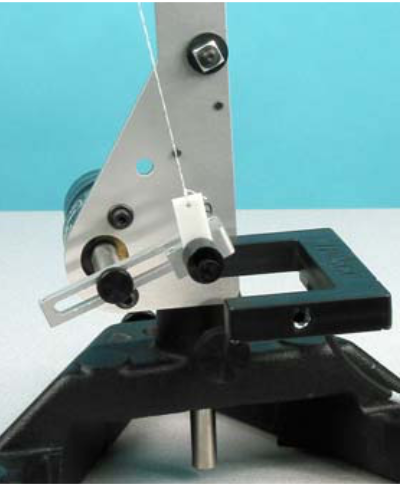
\includegraphics[width = 0.5\linewidth]{images/photogate.png}
    \caption{The photogate used to obtain data for the Poincare section plots}
    \label{fig: photogate}
\end{figure}

After setting up the photogate, we placed two vertical rods on the rod base, and connected them with a cross rod, on which we mounted the rotary motion sensor which would be used to obtain data on the angular position and velocity of the point mass. Next, we used a 1.5-meter-long string to set up the spring mechanism. We threaded the string through the pulley on the rotary motion sensor as shown in Figure \ref{fig: rotary motion sensor and pulley}

\begin{figure}[H]
    \centering
    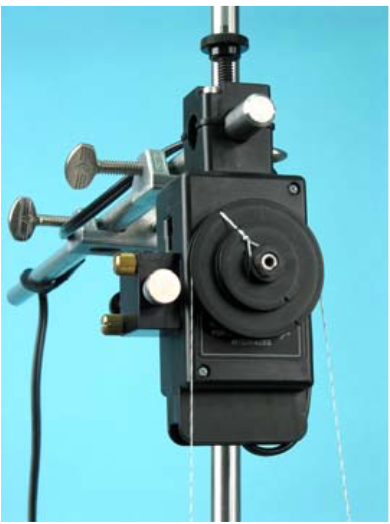
\includegraphics[width = 0.5\linewidth]{images/rotary_motion_sensor.png}
    \caption{The rotary motion sensor and pulley}
    \label{fig: rotary motion sensor and pulley}
\end{figure}

After threading it through the pulley, we attached two springs to each end, and then attached additional sections of string to the opposite ends of each spring. One spring was attached, via the additional section of string, to the motor driver and the other was attached to the leveling screw on the base. We attached the aluminum disk and point mass to the motion sensor, and verified that the spring set-up was constructed so that the tension on either side of the pulley from each spring was equal. 
We then attached the magnet, used to impose damping, onto the rotary motion sensor. This magnet can also be seen in Figure \ref{fig: rotary motion sensor and pulley}. We plugged the driver into the DC power supply, the rotary motion sensor into channels 1 and 2 of the ScienceWorkshop 750 interface, and the photogate into channel 3 of the ScienceWorkshop 750 interface. Using ScienceWorkshop 750, we used the data gathered by the motion sensor and the photogate in a Pasco DataStudio program that made plots of the data. The full set-up is shown in Figure \ref{fig: Full Setup}

\begin{figure}[H]
    \centering
    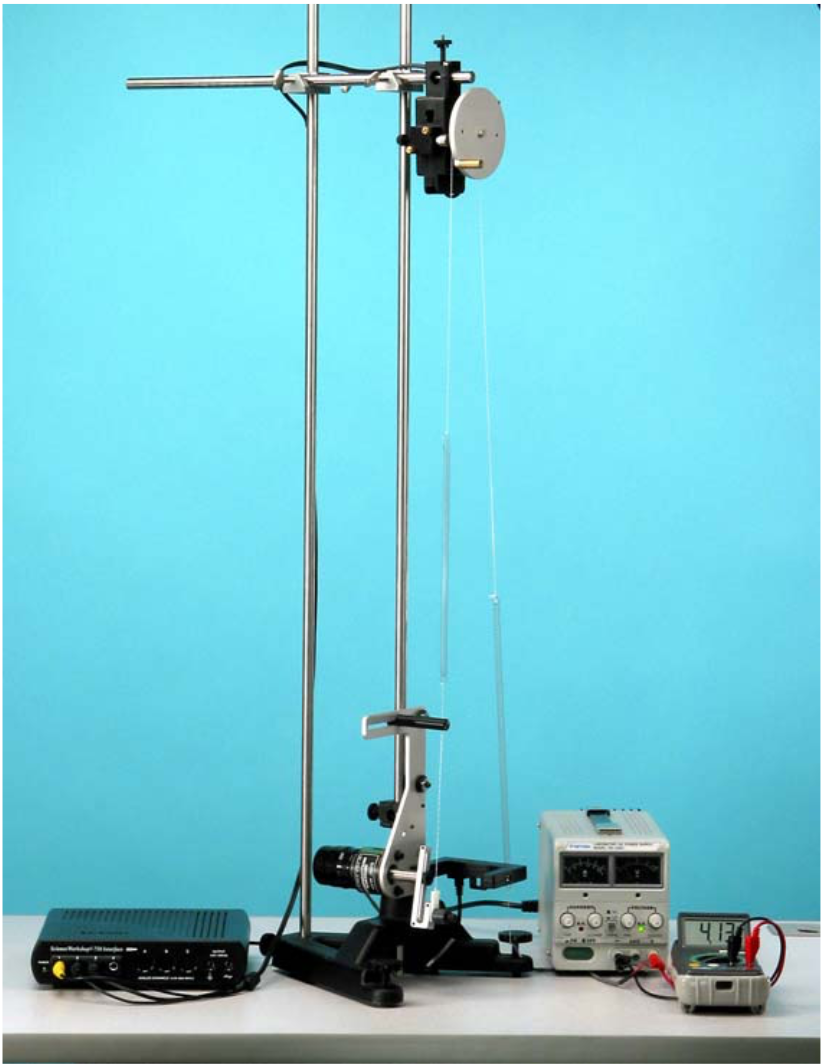
\includegraphics[width = 0.5\linewidth]{images/Full_Setup.png}
    \caption{The full setup for the experiment}
    \label{fig: Full Setup}
\end{figure}

In terms of the methods that we used, we started off by measuring the potential well of our system.
We did so by completely removing any dampening (via screwing the magnet further away from the disk),
and zeroed our angular position so that the point mass is at the 12 O'clock position. This ensures that
the unstable equilibrium is centered at $\theta = 0$. From this, we now rotated the point mass (either clockwise or counter-clockwise) and let go; right as we let go, we also made sure to record the potential
vs. angular position $\theta$. 

We then moved onto measuring the resonant frequency of our pendulum. To do so, we screwed the magnet closer to the disk so that there is now a dampening force acting on the pendulum. We then set the point mass at the 12 O'clock position again and let go of the point mass. Right as we let go, we also made sure to measure the angular velocity vs. time as well as the phase plot. Furthermore, we make sure to plot the FFT of this motion.

Next, we included a driving force on top of the dampening and measured the angular velocity vs. time and phase plot again. We first adjusted the driving force by varying the potential of the motor as well as the driving amplitude. Once the right configurations were made, we were able to start taking data. We made sure to position the point mass at the 12 O'clock position and let go 
of the point mass once the driving arm is at its lowest. On top of the phase plot, we also configured the
program to include the Poincar\'{e} plot and FFT as well. 

Finally, we adjusted the potential of the motor some more until we were able to get the pendulum to be in chaotic motion. We started the measurements the same way that we did in the previous part and measured the same type of relationships. We let the pendulum be in this state for several hours so that we can gather enough data points to make a valid conclusion. Once we gathered the data, we were able to calculate the Lyapunov exponents.

\section{Measurements and Data Analysis}
Figure \ref{fig: Potential Energy Plot} plots the potential energy against the angular position of the pendulum. We see that there are two potential wells corresponding to two stable equilibrium points, as well as one peak corresponding to an unstable equilibrium point at $\theta = 0$. 

\begin{figure}[H]
    \centering
    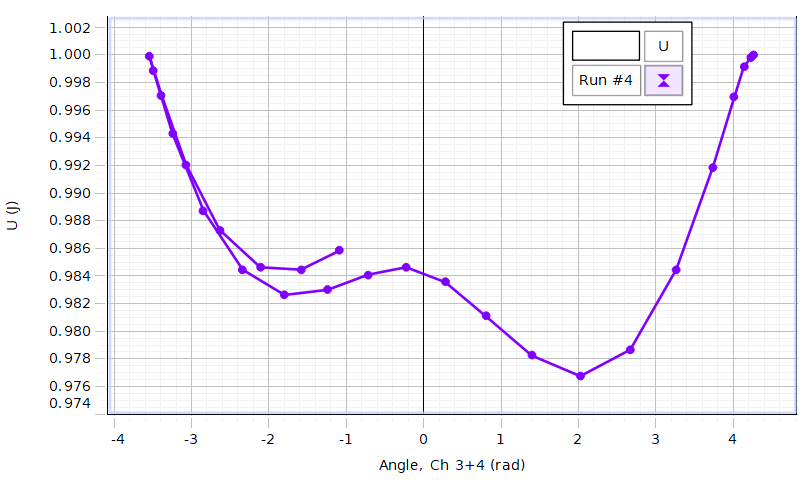
\includegraphics[width = 0.7\linewidth]{images/PotentialWell.PNG}
    \caption{Potential Energy vs. Angular Position}
    \label{fig: Potential Energy Plot}
\end{figure}

Notably, the two potential wells are different sizes because, for any given position of the pendulum, the forces from the two springs are different. This is entirely dependent on the angular position $\phi$ of our driver shaft (confer Figure \ref{fig:apparatus_schematic}). On either side of the unstable point, the pendulum is closer to one spring than to the other, so one spring has a stronger displacement and a stronger force.  

For the next part of the experiment, we measured damped oscillations for the pendulum with no driving force. Here, we see damped sinusoidal oscillations, with the pendulum eventually settling at one of the equilibrium points. The angular velocity converges to zero as shown in Figure \ref{fig: damped undriven pendulum}.

\begin{figure}[H]
    \centering
    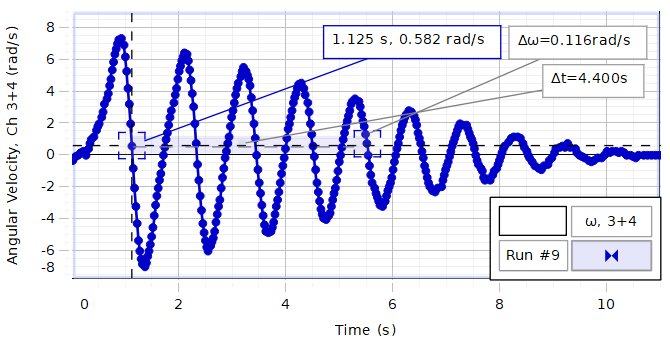
\includegraphics[width = 0.7\linewidth]{images/ResonantFreqOmegavsTime.PNG}
    \caption{Angular Velocity of damped, undriven pendulum over time}
    \label{fig: damped undriven pendulum}
\end{figure}

Looking at this trajectory in phase space, we see the curve takes on a spiral shape that converges to a single point, which is the attractor. This makes sense because eventually, once the pendulum settles at its equilibrium point, $\omega$ reaches zero and $\theta$ reaches some constant value. As we reduced the damping, we noticed that the convergence to the attractor became slower and slower, corroborating the notion that if the oscillations were not damped at all, the curve in phase space would simply be a circle. This makes sense theoretically because if the oscillations were not damped, the angle $\theta$ would vary as a perfect sine function for all times, the angular velocity $\omega$ would vary as a perfect cosine function for all times, so in phase space this would make a perfect circle. This circular attractor is known as a "limit cycle." The phase space plot we discovered is shown in Figure \ref{fig: phase plot damped pendulum}.

\begin{figure}[H]
    \centering
    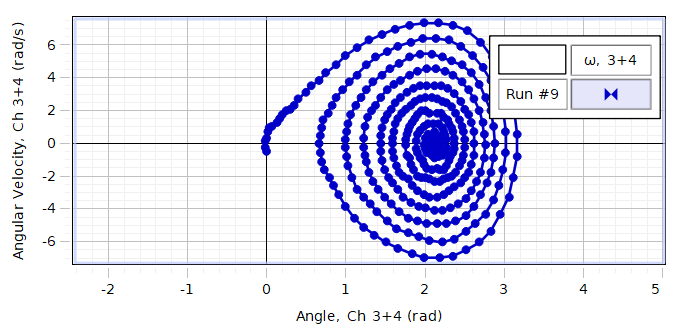
\includegraphics[width = 0.7\linewidth]{images/ResonantFreqOmegavsAngle.PNG}
    \caption{Phase plot of damped, undriven pendulum}
    \label{fig: phase plot damped pendulum}
\end{figure}

Another interesting result from this part of the experiment is the Fast Fourier Transform (FFT), shown in Figure \ref{fig: FFT damped pendulum}.

\begin{figure}[H]
    \centering
    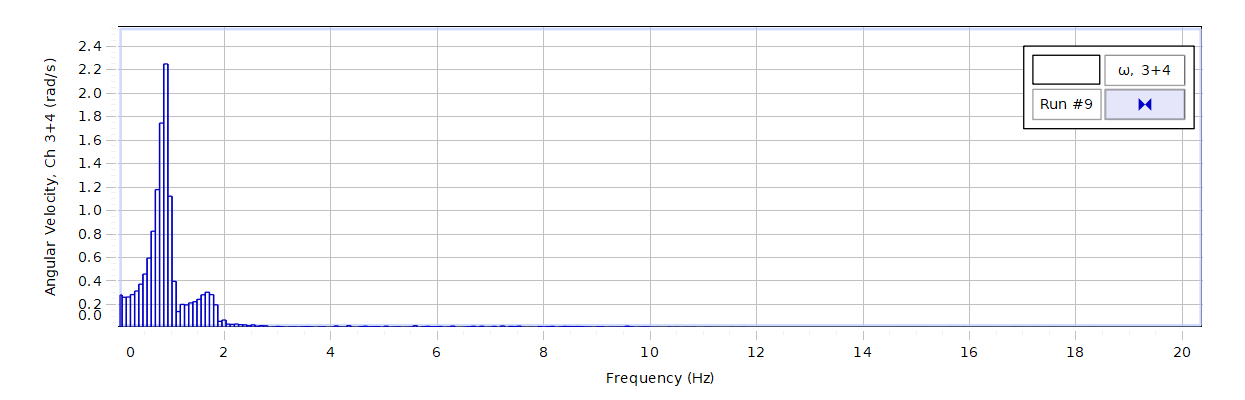
\includegraphics[width = 0.7\linewidth]{images/ResonantFreqFFT.PNG}
    \caption{FFT of damped, undriven pendulum}
    \label{fig: FFT damped pendulum}
\end{figure}

The Fourier Transform deconstructs the motion into its constituent frequencies, and plots which of these are detected with the most intensity. Mathematically, this is tantamount to expanding the motion into a Fourier series, which is a sum of sinusoidal functions each multiplied by a weighting coefficient, given as $\sum_{n} c_{n} \sin(\omega_{n})$. The FFT plots the weighting coefficient for each against $\omega_{n}$. Since the motion followed a sinusoidal curve, we expect there to be a single peak because the Fourier expansions consists of one sine function with the full weight, which is precisely what the plot shows. 

\begin{figure}[H]
    \centering
    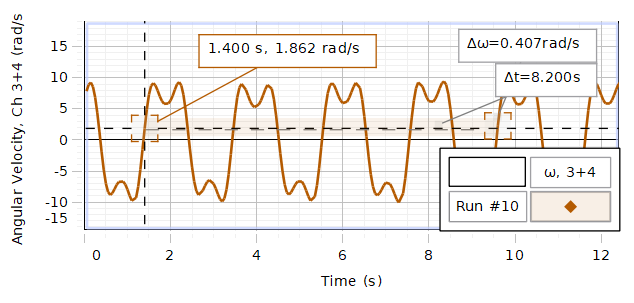
\includegraphics[width = 0.7\linewidth]{images/NonChaoticOmegavsTime.PNG}
    \caption{Angular Velocity of damped, driven pendulum over time}
    \label{fig: damped driven pendulum}
\end{figure}

The next part of the experiment was to add a small driving force. When we did this, the plot of angular velocity $\omega$ vs. time lost its sinusoidal shape, but its motion was still repeated periodically, as shown in Figure \ref{fig: damped driven pendulum}

The introduction of the driving force distorted the sinusoidal motion, while maintaining its periodic nature. This is reflected in the new pattern in phase space. We superimposed the Poincar\'{e} section onto the phase space plot, and we can see that the Poincar\'{e} section is the same point in phase space for each period of the driving force, meaning that the angular velocity $\omega$ and position $\theta$ is the same each period of the driving force. This means that the motion is periodic. The phase space plot with the Poincar\'{e} section is shown in Figure \ref{fig: phase plot damped driven pendulum}.

\begin{figure}[H]
    \centering
    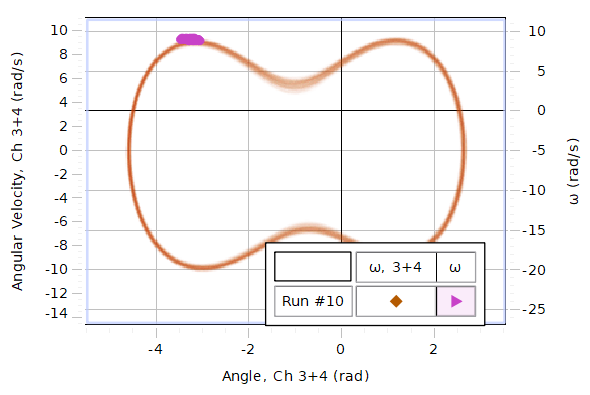
\includegraphics[width = 0.7\linewidth]{images/NonChaoticOmegavsAngle.PNG}
    \caption{Phase plot of damped, driven pendulum}
    \label{fig: phase plot damped driven pendulum}
\end{figure}

This motion makes sense theoretically. When there was no driving force, we started the pendulum at the unstable equilibrium point, and the pendulum fell into one of the two stable equilibrium points depending on which way if fell from the unstable point. This gave it a sinusoidal motion. However, when driving force is added, this force gives the pendulum enough energy to move into the other potential well, where it then experiences another periodic energy boost from the driving force that sends it back to the other potential well, and this continues. Notably, the pendulum never settles at a stable equilibrium point because it is moving back and forth between the two wells. If there were only a single equilibrium point, then the motion would still be sinusoidal because, although the driving force may overcome the damping, the pendulum would still move in the same potential well at the driving frequency. Therefore, this distorted motion is due to the double potential well, which is a consequence of the system's non-linearity. 

\begin{figure}[H]
    \centering
    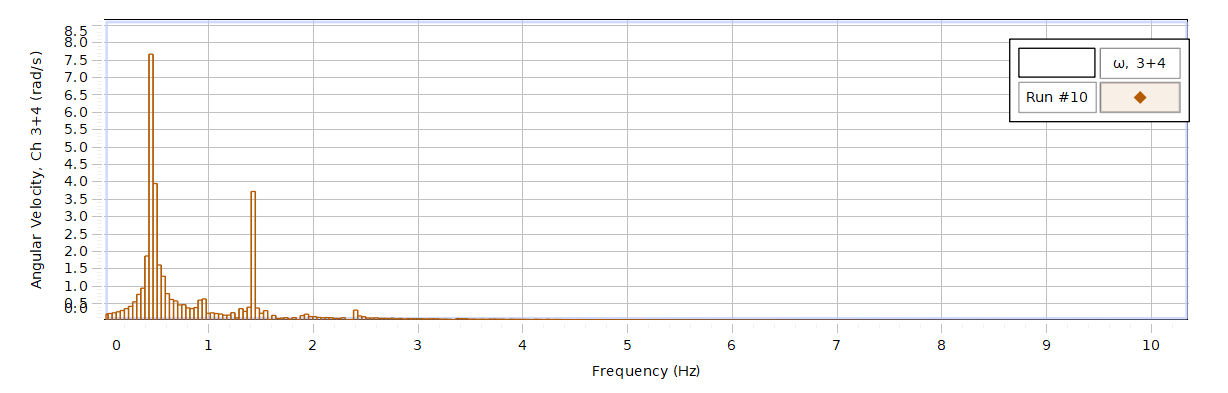
\includegraphics[width = 0.7\linewidth]{images/NonChaoticFFT.PNG}
    \caption{FFT for damped, driven pendulum}
    \label{fig: FFT damped driven pendulum}
\end{figure}

We looked at the FFT for this system as well -- confer Figure \ref{fig: FFT damped driven pendulum}. Here, there appears to be two peak frequencies, indicating that the Fourier expansion of the motion is dominated by two sine functions. One of these functions corresponds to the driving frequency, while the other corresponds to a harmonic frequency. The function that corresponds to the driving frequency is weighted even more heavily, so this is the frequency that corresponds to the taller peak. This explains why our graph of $\omega$ vs. time was distorted from the sinusoidal motion, but still periodic.

For the last part of the experiment, we gradually increased the driving force until we saw chaotic motion. We allowed the pendulum to run for several hours while we collected data. Once again, we superimposed the Poincar\'{e} section on the phase space plot, which is in Figure \ref{fig: chaos poincare and phase plot}.

\begin{figure}[H]
    \centering
    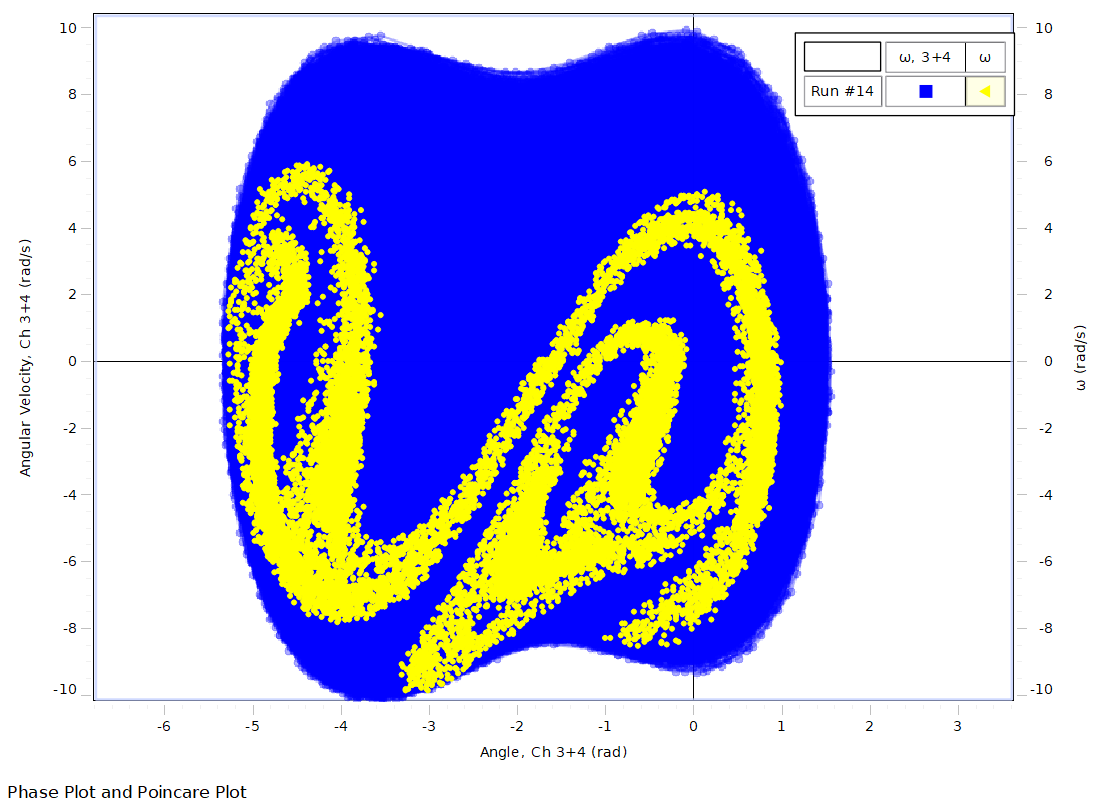
\includegraphics[width = 0.7\linewidth]{images/ChaoticPlot3.PNG}
    \caption{Phase and Poincar\'{e} plot of our chaotic run.}
    \label{fig: chaos poincare and phase plot}
\end{figure}

The Poincare section we see here looks like the strange attractor we expected. While we were not capable of collecting enough data to look at fractal behavior, we do see that the motion is not periodic or predictable. The motion is chaotic because the angular velocity $\omega$ and angular position $\theta$ change sporadically with the period of the driving force. 

We also looked at the FFT for this, and noted that there are many peaks for on the FFT plot for chaotic motion, indicating a long Fourier expansion with many prominent frequencies, as shown in Figure \ref{fig: FFT chaos}. 

\begin{figure}[H]
    \centering
    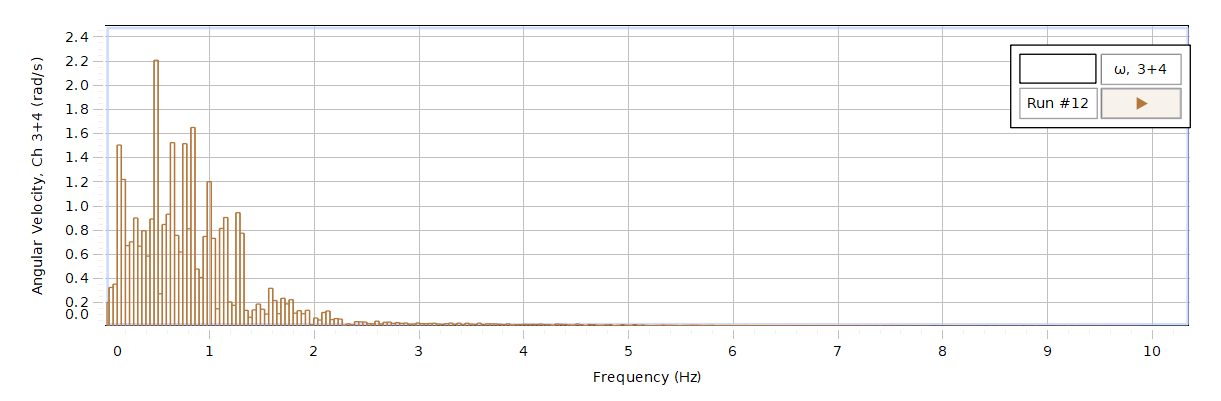
\includegraphics[width = 0.7\linewidth]{images/ChaoticPlot1FFT.PNG}
    \caption{FFT for chaos run}
    \label{fig: FFT chaos}
\end{figure}

Finally, we can calculate the Lyapunov constants for both the chaotic and non-chaotic motions. To do this, we found two points in the Poincare plot that were close together and calculated the distance between them in the phase plane using the formula $\sqrt{\theta^{2} + \omega^{2}}$. Then, we computed the distance between the two points for several subsequent periods of the driving force. Equation \ref{eq:11} implies $\lambda t = \ln \lvert \frac{\delta \mathbf{u} (t)}{\delta \mathbf{u} (0)} \lvert$. Therefore, we plot the natural log of the ratio of the subsequent distances with the initial distance over time, taking the slope to be our Lyapunov exponent value. After doing so, we get the following Lyapunov exponents: $-5.94 \times 10^{-3} \pm 4.38 \times 10^{-3}$ for the non-chaotic motion and $1.35 \pm 4.38 \times 10^{-3}$ for the chaotic motion. All of this can can be shown in Figures \ref{fig:NonChaotic Lyapunov}, \ref{fig:NonChaotic Lyapunov Stats}, \ref{fig:Initial Chaotic Lyapunov}, and \ref{fig:Full Chaotic Lyapunov}. Specifically, 
\ref{fig:NonChaotic Lyapunov} shows that the separation between the two points does not change exponentially with time, as we would expect from a non-chaotic system. The separation is bounded by the size of the cluster of points in the Poincar\'{e} section in \ref{fig: phase plot damped driven pendulum}. For the chaotic case, we see in \ref{fig:Full Chaotic Lyapunov} that the separation between the two points does increase exponentially until it saturates. Eventually, the distance between the two points approximates the scale of the attractor, at which point the separation stops increasing exponentially through in time. This saturated portion of the curve is not included when computing the Lyapunov exponent. \ref{fig:Initial Chaotic Lyapunov} shows these points.   
\begin{figure}[H]
    \centering
    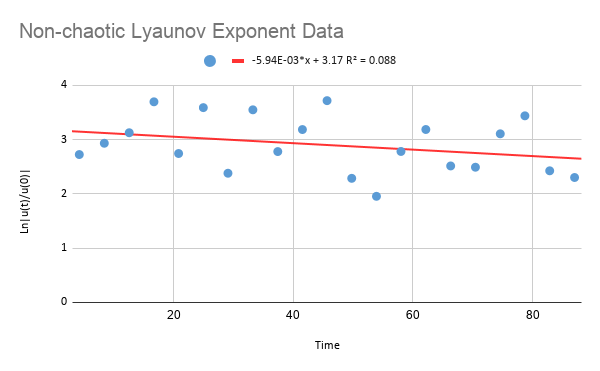
\includegraphics[ width = 0.7\linewidth ]{images/Non-chaotic Lyaunov Exponent Data.png}
    \caption{Lyapunov exponent data for non-chaotic motion}
    \label{fig:NonChaotic Lyapunov}
\end{figure}

\begin{figure}[H]
    \centering
    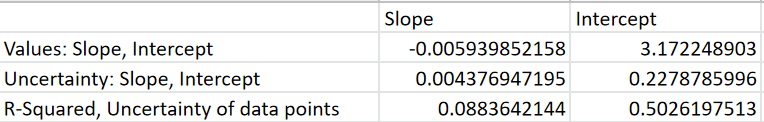
\includegraphics[ width = 0.8\linewidth ]{images/Non-chaotic Lyaunov Exponent Stats.png}
    \caption{Measurements and Uncertainties for non-chaotic Lyapunov exponent}
    \label{fig:NonChaotic Lyapunov Stats}
\end{figure}

\begin{figure}[H]
    \centering
    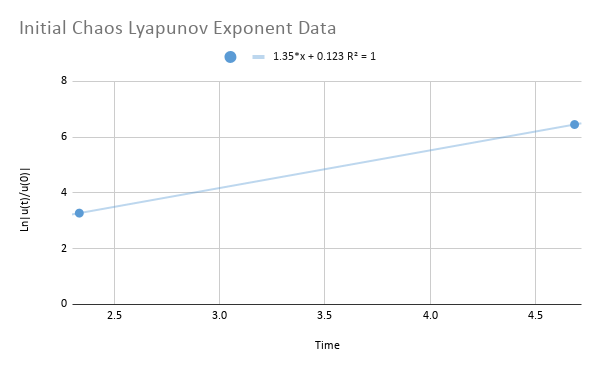
\includegraphics[ width = 0.7\linewidth ]{images/Initial Chaos Lyapunov Exponent Data.png}
    \caption{Initial Lyapunov exponent data for chaotic motion}
    \label{fig:Initial Chaotic Lyapunov}
\end{figure}

\begin{figure}[H]
    \centering
    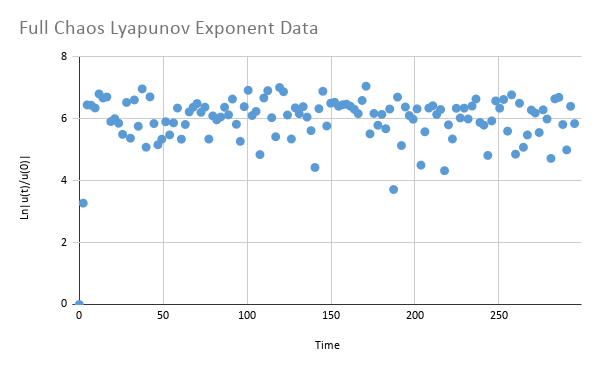
\includegraphics[ width = 0.7\linewidth ]{images/Full Chaos Lyapunov Exponent Data.png}
    \caption{Full Lyapunov exponent data for chaotic motion}
    \label{fig:Full Chaotic Lyapunov}
\end{figure}

\section{Discussion}
Many of our discoveries were consistent with what we expected to see from the theory. The undriven damped motion took on the decaying sinusoidal pattern that we'd expect, converging to a single equilibrium point represented by the fixed point attractor in phase space. Once we added the driving force, the slightly distorted, but still periodic, motion was consistent with the FFT and double potential well. The chaotic attractor we found is also very consistent with that discovered in other research. 

Additionally, the Lyapunov exponents that we found were plausible. For the chaotic motion, we found a that $\lambda \approx 1.35$ with an uncertainty of $4.38 \times 10^{-3}$. We make note that we used the same uncertainty as in the non-chaotic case -- this is because the distance between our two test points saturated extremely quickly, so we were only left with two data points to look at. As a result, we found it appropriate to use the uncertainty value for the non-chaotic case (as there was no other choice), so there is not much that we can say with confidence. However, the results that we got still held up with what we expected to see. Taking two points that are initially very close together, their separation distance scales as $\exp(\lambda t)$. Therefore, $\lambda > 1$ means that the points rapidly diverge, which is characteristic of chaotic motion. This is what we found. For the non-chaotic case, we found that the Lyapunov exponent was very close to zero -- $-5.94 \times 10^{-3} \pm 4.38 \times 10^{-3}$ to be exact -- which means that the separation between the points did not change very much. We expected this to be the case since our motion was periodic; in a perfect scenario, we should expect the Poincar\'{e} plot to be a single point. However, we ended up with a cluster of points instead, but we still have that zero is within our confidence interval (which is $( -1.47 \times 10^{-2}, 2.82 \times 10^{-3})$). Although close to zero, it is worth noting that our result for this exponent was slightly negative, indicating that the distance between the points actually decreased, which is characteristic of non-chaotic systems with a stable attractor, such as this pendulum with a small driving force. 

Some reasons for how we could have done the experiment better was to choose parameters (e.g. driver voltage, driver amplitude, dampening, etc.) such that our pendulum transitioned into chaotic motion slower; this way, we could gather more data points and offer a confidence interval. Furthermore, we note that friction was notable in our motor, which could have been what caused our driver arm to not rotate at a constant rate. As a result, this introduced noise/uncertainty in our Poincar\'{e} data, and is why we did not have our Poincar\'{e} plot to be a cluster of points rather than a single for our non-chaotic motion.

One phenomenon that we unfortunately were unable to detect was period doubling on the route to chaos. The motion of the pendulum was periodic and non-chaotic for a small value of the driving force. We increased the driving force gradually and found that the motion turned chaotic after passing a certain threshold of the driving force. We expected that as we gradually increased the driving force, there would be some distortion of the motion before the abrupt change to chaos, as this is what much of the theory predicts. Specifically, once the parameter being varied (in this case, the driving force) passes a certain threshold called a period-doubling bifurcation. At this point, a new motion emerges with double the period of the initial trajectory. As we increase the parameter even more, the period continues to double until we reach motion that is effectively aperiodic. This infinite sequence of period doubling is called a period doubling cascade. This is the phenomenon we were unable to detect. 

There are several possible explanations for this. For instance, the DC power supply limited how finely we could adjust the voltage which controlled the driving motor, so perhaps we overshot the bifurcations even with our gradual adjustments. Additionally, the friction we noticed in the driving motor, which we discussed above, may have unpredictably impacted the period of the driving force, which in turn prevented us from isolating the period doubling bifurcation as we increased this force. 

Since we measured the points on Poincar\'{e} plot once every period of the driving force, the fact that the driving period varied due to friction in our driving motor lead to uncertainty in those Poincar\'{e} points, which in turn lead to uncertainty in our estimates for the Lyapunov exponents, as discussed above.  

Another phenomenon we were unable to detect was the fractal geometry of the attractor. This was simply due to limitations in the number of data points we were able to collect in the Poincar\'{e} section. If we had collected more, then we would have been able to zoom in on the attractor and see self-similar behavior on small scales. This experiment could be improved by taking data on a machine with larger computing power that would be able to collect enough points to exhibit fractal behavior on the Poincare section. 

The chaotic behavior that we saw here has a number of applications, many of which have nothing to do with mechanics. In fact, one of the pioneers of chaos theory, Edward Lorenz, came across the phenomenon when studying weather predictions. He wished to study a very long data sequence, but in order to simplify his procedure, he began the simulation at the halfway point in order to study the second half. The computer that he was using, a Royal McBee, stored six digits in his memory but, thinking it would not have a significant effect, Lorenz only entered three digits as the initial conditions. He discovered that this roundoff error made a huge difference in the ultimate trajectory \cite{History}. He therefore concluded that long-range weather prediction was not feasible because the governing equations were chaotic and exhibited extreme sensitivity to initial conditions\cite{weather}. 
Lorenz would then go on to formulate a specific chaotic system called the Lorenz system as an additional example of how chaotic behavior arises in the modelling of many phenomena. Specifically, this was a model for atmospheric convection \cite{weather}. The Lorenz system is given by the following three equations:

\begin{equation}
    \frac{dx}{dt} = \sigma(y-x)
\end{equation}

\begin{equation}
    \frac{dy}{dt} = x(\rho - z) - y
\end{equation}

\begin{equation}
    \frac{dz}{dt} = xy - \beta z
\end{equation}

Lorenz discovered that this system is also chaotic because it exhibits extreme sensitivity to initial conditions as well as a strange attractor when the solution is plotted in phase space. This attractor exhibits fractal geometry and is known for its reminiscence of a pair of thin butterfly wings. In fact, the term "butterfly effect" stems from this discovery. This attractor is shown in Figure \ref{fig: Attractor of Lorenz system}.  

\begin{figure}[H]
    \centering
    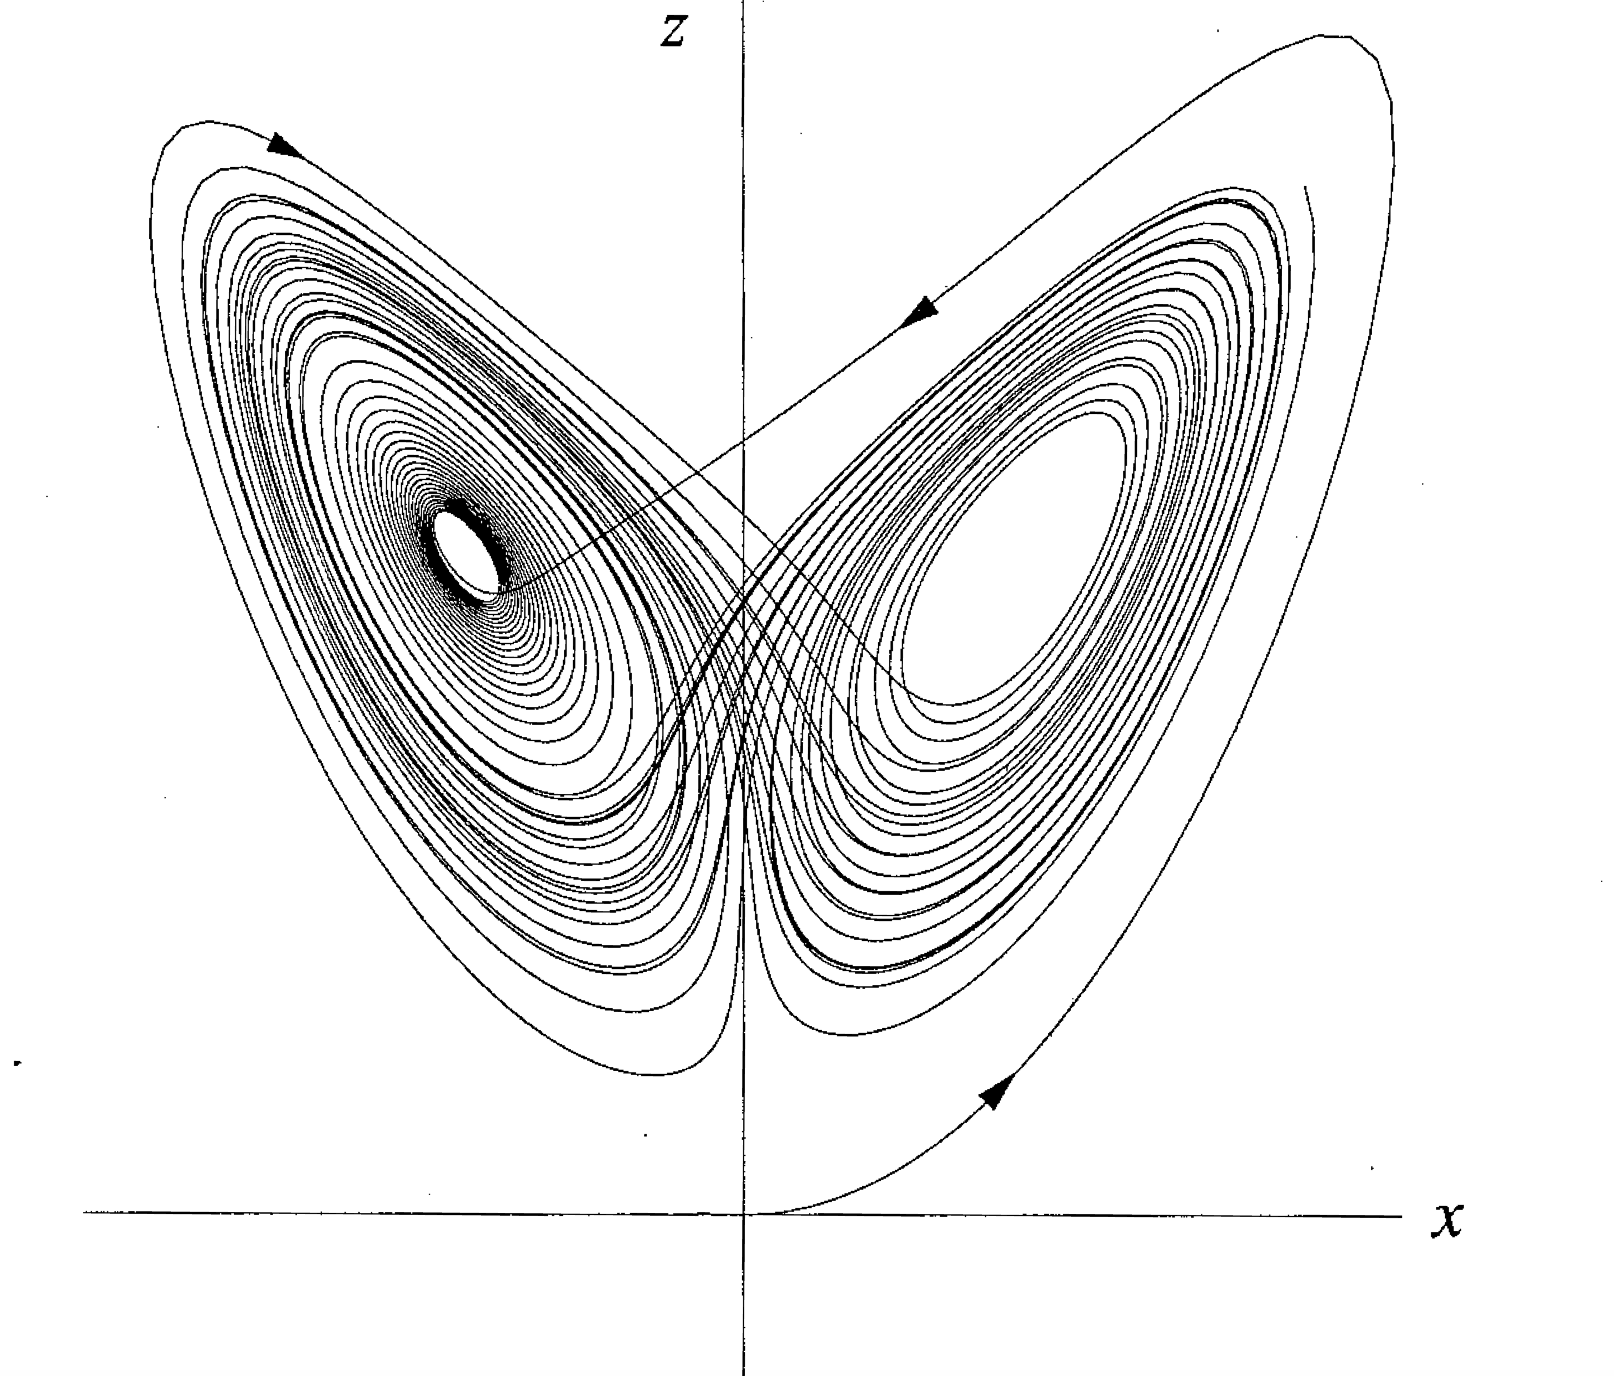
\includegraphics[width = 0.7\linewidth]{images/Butterfly curve.png}
    \caption{Attractor of Lorenz System}
    \label{fig: Attractor of Lorenz system}
\end{figure}

The Lorenz system gives rise to another fascinating application of chaos theory, which involves using chaos to send coded messages. The premise involves masking a message with much louder chaos, and then sending it to a receiver which can subtract that added chaos and recover the original message \cite{Strogatz}. Chaos was added using the circuit shown in Figure \ref{fig: circuit used to generate chaotic mask}. 

\begin{figure}[H]
    \centering
    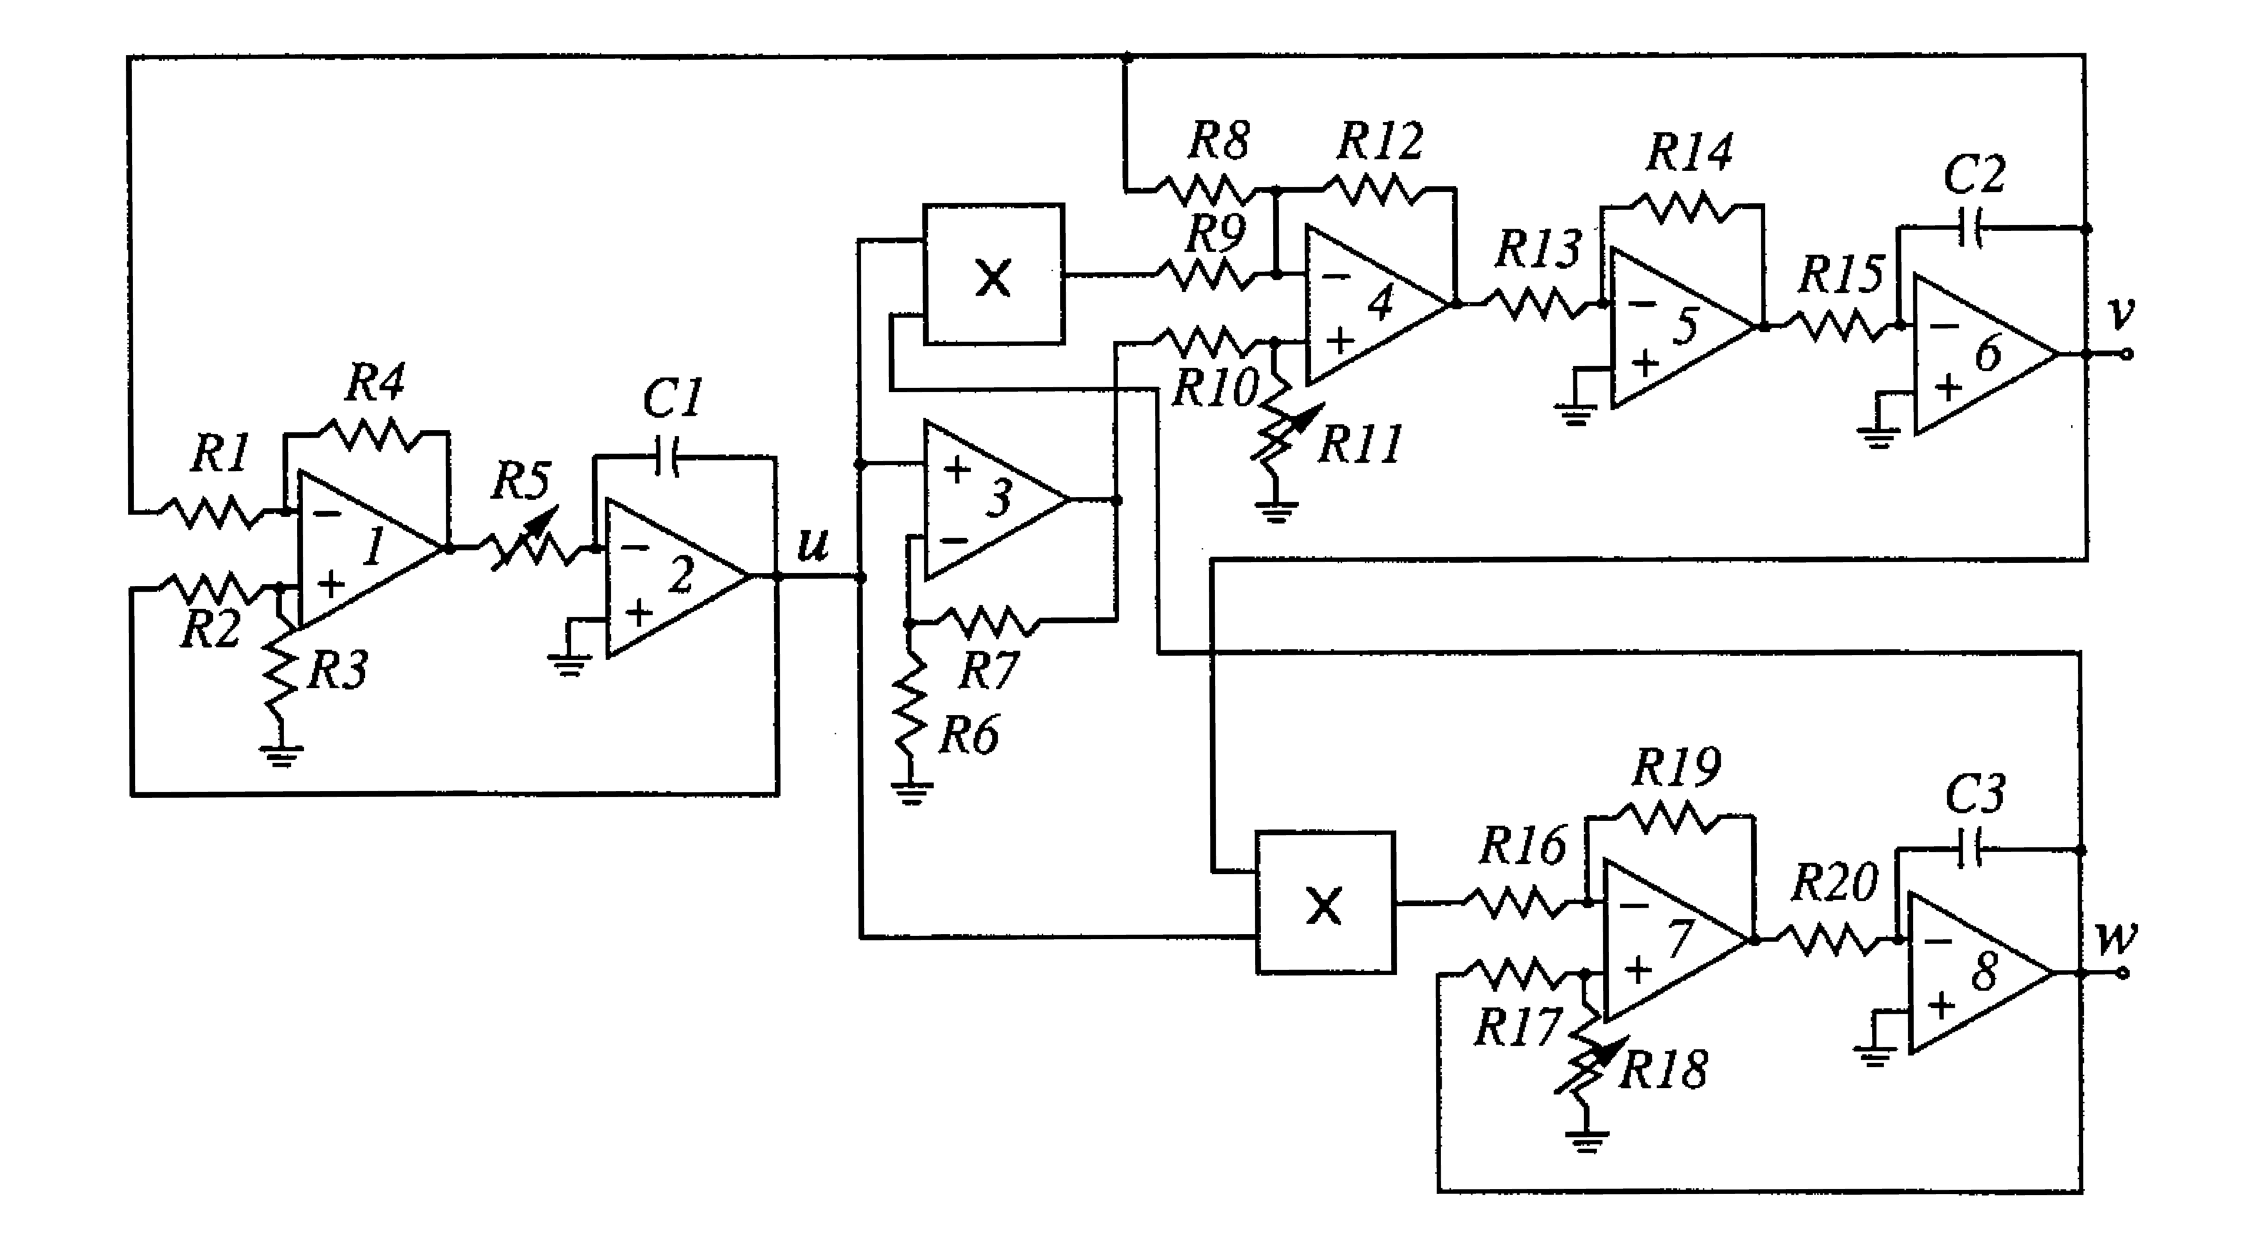
\includegraphics[width = 0.7\linewidth]{images/Circuit.png}
    \caption{Circuit used to generate chaotic mask}
    \label{fig: circuit used to generate chaotic mask}
\end{figure}

There are three voltages in this circuit, denoted $u$, $v$, and $w$, which are governed by the Lorenz equations. If one listens to the signal from the circuit through a loudspeaker, they would hear static, indicative of chaotic behavior. Then, the signal from this circuit was sent to a receiver, which consisted of an identical circuit driven by the signal from the transmitting circuit. This produced "synchronized chaos," which refers to the fact that the chaotic signal from the receiving circuit was almost identical to that of the transmitting signal. Electronic subtraction was used to remove the chaotic mask from the receiver signal and recover the original sound \cite{Strogatz}. Figure \ref{fig: frequencies used for chaotic signal masking} illustrates the frequencies that were utilized.

\begin{figure}[H]
    \centering
    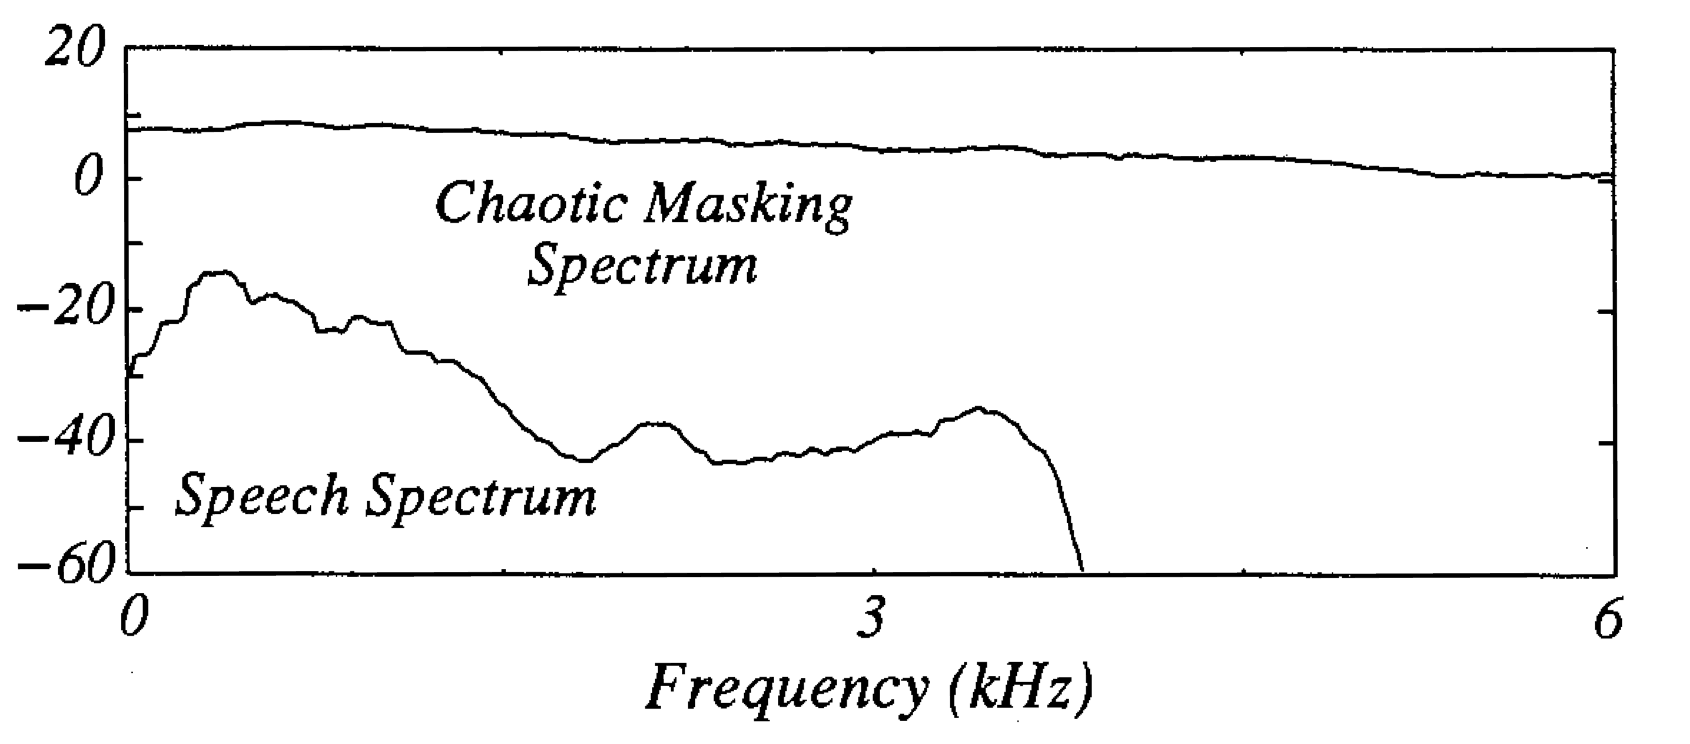
\includegraphics[width = 0.7\linewidth]{images/Frequency.png}
    \caption{Frequencies used for chaotic signal-masking}
    \label{fig: frequencies used for chaotic signal masking}
\end{figure}

These are only a few examples of applications of the chaotic theory that we studied in this experiment. Additional examples include a chaotic version of the particle swarm optimization (PSO) algorithm to predict gas solubility in the context of polymer manufacturing \cite{chemistry} and recurrence quantification analysis (RQA) in the context of economic modeling \cite{economics}. 

\section{Conclusion}
In this experiment, we studied non-chaotic and chaotic motion. As shown in Figure \ref{fig: phase plot damped driven pendulum}, we found the phase plot of the non-chaotic motion to be a closed limit cycle, and the corresponding Poincar\'{e} plot was a cluster of points. This was to be expected since the non-chaotic motion was periodic. Furthermore, the FFT showed two peak frequencies (as well as some additional smaller frequencies) which corresponds the driver frequency and the subsequent harmonic frequencies. This is also expected as we see in Figure \ref{fig: Potential Energy Plot} that we have two potential wells -- more importantly, our potential is not quadratic. Rather, it is more likely that it is of order 4. Hence, we should not get only one frequency peak (corresponding to pure sinusoidal motion -- i.e. quadratic potential), but should get several (corresponding to the harmonic frequencies of our main driver frequency).

As for chaotic motion, we look at Figure \ref{fig: chaos poincare and phase plot}. The section in blue corresponds to the phase plot, and indicates to us that there is no limit cycle or any other conventional fixed point attractor. We expected this to be the case for chaotic motion. The corresponding Poincar\'{e} plot also shows us that the motion is aperiodic as we measure a different angular velocity for every period. Looking at the FFT of the chaotic motion, we see that there are many noticeable frequency peaks. Again, this is expected since the motion is chaotic, and we expect the system to cover a wide range of frequencies as a result.

To show the difference between chaotic and non-chaotic quantitatively, we calculate the Lyapunov exponents. Doing so, we found the Lyapunov exponent for the non-chaotic motion to be $-5.94 \times 10^{-3} \pm 4.38 \times 10^{-3}$ and we found it to be $1.35 \times 10^{-3} \pm 4.38 \times 10^{-3}$ for the chaotic motion. We expect the Lyapunov constant to be zero for the non-chaotic motion, and greater than 1 for chaotic motion. This is exactly what we see, but we should note that our chaotic motion data only had two data points due to how fast the distance between our two test points exponentially diverged. As a result, we were not able to obtain any uncertainty values for our chaotic motion run; thus, we had to resort to using the uncertainty from our non-chaotic run. However, we have zero to be within our confidence interval for the non-chaotic motion run.

As for how our experiment could be potentially improved in the future, we could start out by switching out the motor for one that operates with lower friction. This would help our driver period to remain constant all throughout the run. We could also reduce the wobble of the apparatus by anchoring it down more effectively. This would help reduce the interference that our apparatus produces with the motion of the pendulum. 

\section{References for Figures}
Figures \ref{fig:apparatus_schematic} and \ref{fig: phase space plot} can be found on page 2 and 7 of \cite{floridalab}, respectively. Furthermore, Figures \ref{fig: sine linear theta vs time plot}, \ref{fig: sine phase space plot}, and \ref{fig: sine wave phase space attractor} can all be found on page 8 of \cite{floridalab}. Lastly, Figure \ref{fig: Chaotic Poincare section graphs} can be found on page 10 of \cite{floridalab}

Figures \ref{fig: photogate}, \ref{fig: rotary motion sensor and pulley}, and \ref{fig: Full Setup} can all be found on page 3 of \cite{pascolab}. Figures \ref{fig: Attractor of Lorenz system}, \ref{fig: circuit used to generate chaotic mask}, and \ref{fig: frequencies used for chaotic signal masking} can be found in chapter 9 of \cite{Strogatz}.

\bibliographystyle{unsrt}
\bibliography{References}

\end{document}
